\section{Mise en contexte}

\begin{frame}
    \begin{center}
    \vspace{0.5cm}
    \boxed{
        Mise en contexte
    }
    \end{center}
\end{frame}

\begin{frame}
    \frametitle{Mise en contexte - Aperçu historique}
    \begin{columns}
        \column{0.38\linewidth}
        \centering
        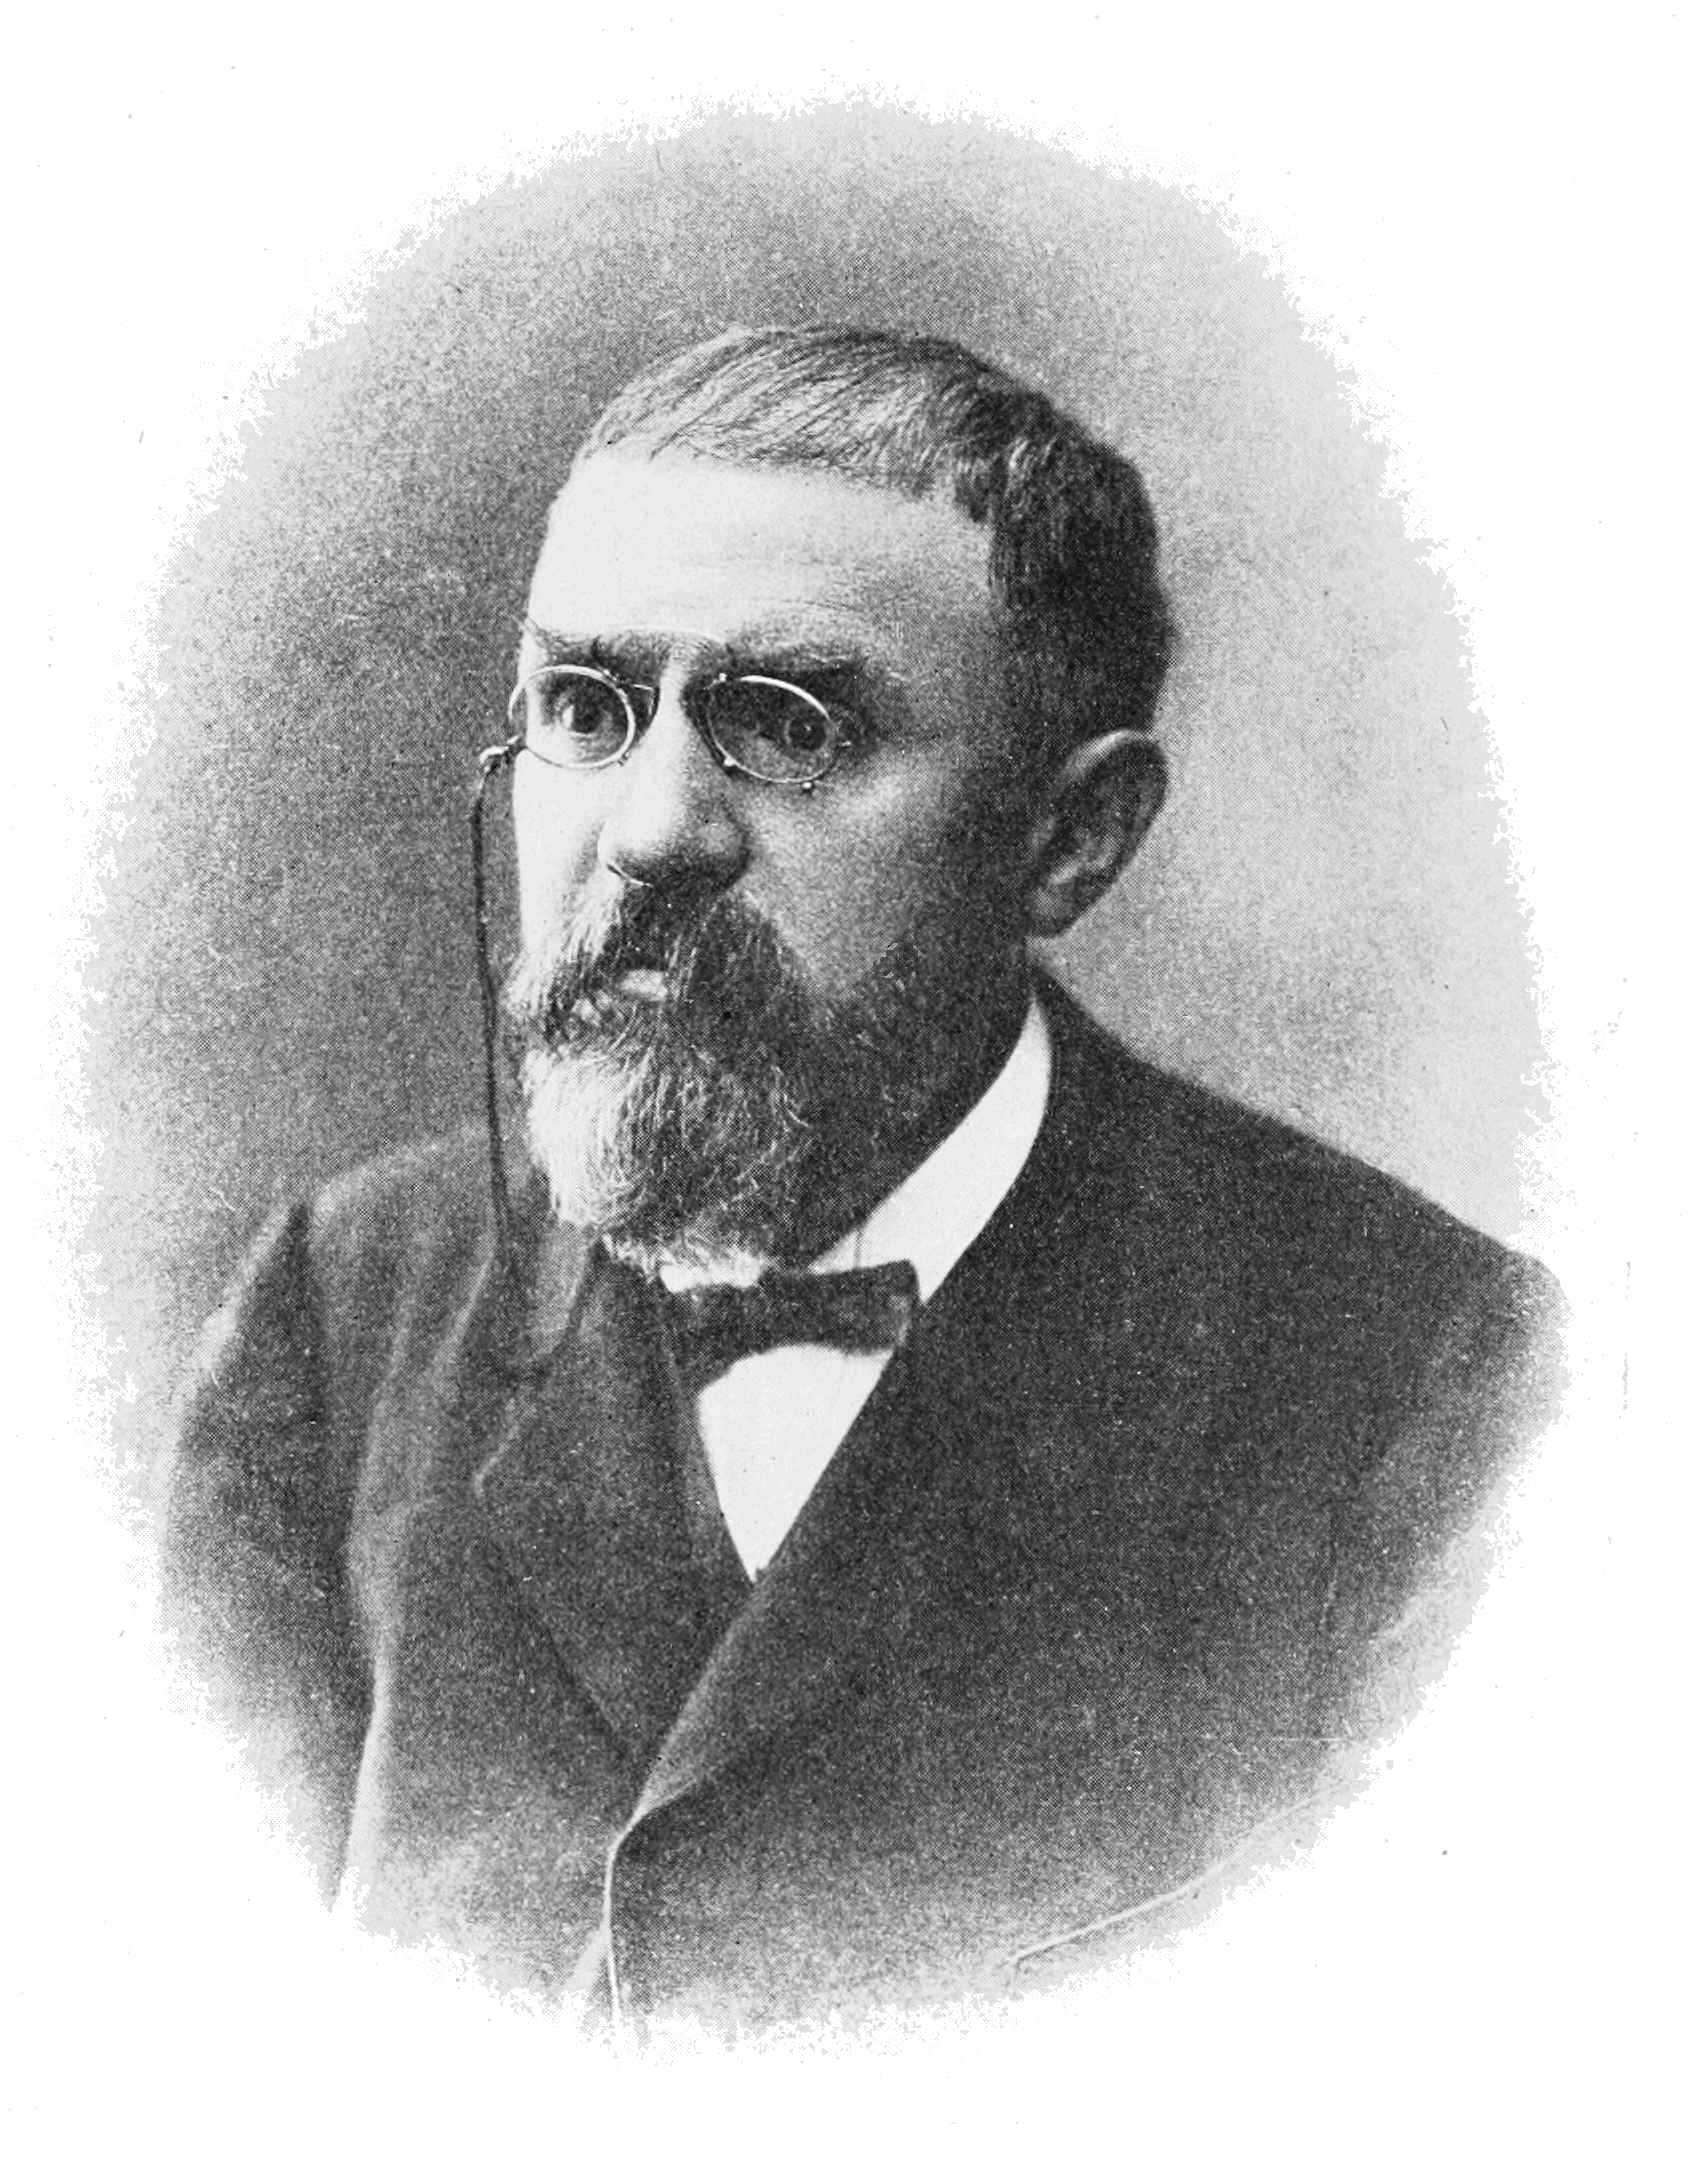
\includegraphics[scale=0.06]{figures/henri_poincare.png}
        \column{0.58\linewidth}
        \textit{"\dots it may happen that small differences in the initial conditions produce very great ones in the final phenomena. A small error in the former will produce an enormous error in the latter. Prediction becomes impossible\dots"} - in a 1903 essay Science and Method.
    \end{columns} 
\end{frame}

\begin{frame}
    \frametitle{Mise en contexte - Définitions}
    \begin{itemize}
        \setlength\itemsep{1em}
        \item[$\diamond$] Émergence des systèmes dynamiques (climat, biologie, etc.) \\
        \item[$\diamond$] Systèmes d'équations différentielles \\
        % \item[$\diamond$] Étude des solutions dans l'espace des phases (sous-ensemble)
    \end{itemize}
    \vspace{0.5cm}
    \begin{defblock}{Définition: Attracteur}
        L'attracteur est un sous-ensemble de l'espace des phases vers lequel les solutions convergent sous certaines conditions initiales.
    \end{defblock}
\end{frame}

\begin{frame}
    \frametitle{Mise en contexte - Définitions}
    Condition de validité d'une condition initiale appartenant à l'attracteur
    \vspace{0.5cm}
    \begin{defblock}{Définition: Bassin d'attraction}
        Soit un attracteur $A$, son bassin d'attraction $W_A$ est donné par
        \begin{align}
            W_A = \{r\in R\;\;| \lim_{t\to\infty}f(r, t)\in A\},
        \end{align}
        où $r$ est un point de l'espace des phases $R$ et $f(r, t)$  une solution de l'attracteur $A$.
    \end{defblock}
\end{frame}

